\chapter{Introdución}
\label{chap:introducion}


\lettrine{E}{n} economía se entiende por venta \textquote{la entrega de un determinado bien o servicio bajo un precio estipulado o convenido y a cambio de una contraprestación económica en forma de dinero por parte de un vendedor o proveedor}~\cite{ventas}. Por lo tanto la realización de ventas supone el núcleo de la actividad económica de un gran margen del espectro económico, donde los actores económicos obtienen ganancias dinerarias tras la entrega de un producto o servicio en el que se especializan. El proceso de venta culmina con la concreción de transacción de venta efectiva ~\cite{proceso-venta}, por lo que una vez realizada dicha transacción es necesario disponer de una herramienta que permita registrar dicha venta, esto es, la relación entre lo que se ha vendido, a quién, cuando y por qué importe.

Con el objetivo de diseñar y desarrollar una aplicación que le permita a una empresa gestionar su catálogo de productos y servicios, así como la cartera de clientes y los productos y servicios que han contratado dichos clientes a lo largo de su vinculación con la empresa nace este trabajo. Se trata de un software de \gls{opensource} desarrollado bajo licencia \acrfull{licencia} con el objetivo de cumplir con las cuatro libertades esenciales de los usuarios:
\begin{itemize}
\item Libertada para ejecutar el programa sin restricciones.
\item Libertad para estudiar y modificar el código.
\item Libertad para redistribuir copias exactas.
\item Libertad para distribuir versiones modificadas.
\end{itemize}

Esto permitirá que el software presentado en este \acrfull{tfg} pueda ser adaptado a las distintas necesidades del usuario a través de las modificaciones software necesarias siempre que se cumpla con los acuerdos de licencia bajo los que se ha desarrollado. Para tal fin se ha creado un repositorio en la web de Github que contiene tanto la presente memoria como el código desarrollado para este \acrshort{tfg}. Dicho repositorio se encuentra disponible en \url{https://github.com/cgcgit/CoMaSw.git} y está estructurado de la siguiente manera:
\begin{itemize}
\item Carpeta \emph{\textbf{CoMaSw}}: contiene el código fuente generado.
\item Carpeta \emph{\textbf{memoria}}: contiene los ficheros .tex generados y los recursos necesarios para la elaboración de la presente memoria.
\end{itemize}

Hemos optado por referirnos genéricamente a esta herramienta como un software de gestión de contratación, ya que su principal función es la de mantener el catálogo de productos y servicios a ofertar por la empresa así como gestionar la contratación de los mismos por los distintos clientes de dicha empresa. Evitamos así el uso de los términos más familiares de \acrfull{crm} y \acrfull{erp} puesto que sus funcionalidades van mucho más allá de las mencionadas para la herramienta desarrollada, englobando todos los sistemas informáticos de apoyo a la gestión de procesos empresariales, cada uno con su propio enfoque: el primero se centra en mejorar las ventas mientras que el objetivo del segundo es reducir costes aumentando la productividad.


\section{Motivación}
\label{sec:motivacion}

El proyecto \emph{``Software de gestión de contratación con arquitectura Java EE multicapa para empresas proveedoras de servicios''} surge de aunar el deseo de desarrollar una aplicación web como parte del \acrshort{tfg} de la titulación y el conocimiento adquirido durante la labor de soporte realizada en un sistema de facturación de una empresa proveedora de servicios.

Visto a muy alto nivel, los procesos de negocio se pueden definir en tres fases tal y como se muestra en la \figurename~\ref{fig:fases-proceso-negocio} 

\begin{figure}[hp!]
  \centering
  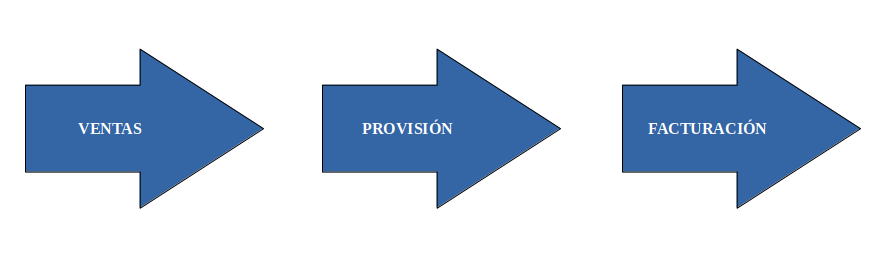
\includegraphics[width=0.50\textwidth]{imaxes/fases-proceso-negocio.png}
  \caption{Fases del proceso de negocio}
  \label{fig:fases-proceso-negocio}
\end{figure}

\begin{itemize}
\item \textbf{Venta}: conjunto de actividades orientadas a realizar y formalizar la venta de un servicio a través de la contratación del mismo.
\item \textbf{Provisión}: conjunto de actividades cuya finalidad es la de proveer el servicio previamente contratado al cliente.
\item \textbf{Facturación}: comprende todas las actividades destinadas a facturar la prestación de los servicios contratados y provisionados y realizar la posterior puesta a cobro de los mismos.
\end{itemize}

Como ya hemos indicado, la herramienta desarrollada para este \acrshort{tfg} se centrará en la fase de venta, concretamente la correspondiente a registrar la venta y gestionar los productos y servicios contratados así como el catálogo de productos y servicios de la empresa.


\section{Definición de objetivos}
\label{sec:objetivos}


El objetivo primordial del presente proyecto es diseñar y desarrollar una aplicación 100\% \gls{opensource} que permita gestionar el catálogo de productos y servicios de una empresa así como la cartera de clientes y sus contrataciones, para lo que se tendrán en cuenta una serie de elementos parametrizables (esto es, modificables según las necesidades del sistema) que conformarán la definición de las entidades a manejar por el sistema.

Además de realizar las diferentes altas, bajas y modificciones de los elementos que conforman el catálogo de productos y servicios y la cartera de clientes, la aplicación desarrollada deberá gestionar el histórico de datos para los elementos susceptibles de cambio y así poder reflejar los continuos cambios derivados que puedan sufrir (cambio de precio en entidades facturables, modificación del servicio contratado, cambios en las tasas impositivas de los mismos, etc). También contará con funcionalidades para la gestión de los usuarios de la plataforma, permitiendo dar de alta usuarios nuevos así como modificar o eliminar usuarios existentes. Asimismo permitirá que cualquier usuario de la plataforma pueda cambiar sus datos de contacto o su contraseña.

La herramienta a desarrollar será una aplicación web, lo que permitirá un ahorro en recursos (ya que para su ejecución sólo es necesario un equipo con acceso a internet y un navegador instalado) y facilitará su distribución, ya que se evita el proceso de descarga de actualizaciones: cualquier modificación realizada en el software estará disponible para el usuario simplemente accediendo a la aplicación.

Durante el desarrollo de este \acrshort{tfg} se ha tenido en mente el sector \acrshort{tic} de las operadoras de telefonía, ya que, como se ha indicado anteriormente, se ha querido aprovechar el conocimiento adquirido a través de la experiencia profesional, aunque podría adaptarse a cualquier otra empresa cuyo modelo de negocio se base en suscripciones con tarifas periódicas (por ejemplo gimnasios, academias de idiomas, etc...).


\section{Estructura de la memoria}
\label{sec:estructura}

La presente memora se estructura en 9 capítulos, 2 anexos y una bibliografía:

\begin{itemize}
\item El capítulo \ref{chap:introducion} se corresponde al presente capítulo, en el que se realiza una descripción general del proyecto
introduciendo las ideas principales y el escenario sobre el que nos encontramos.
\item El capítulo \ref{chap:estado-arte} se centra en el estudio del arte, en que se exponen distintas herramientas relacionadas con el tema central así como sus características principales.
\item El capítulo \ref{chap:teoria} muestra una introducción al procesos de negocio y los distintos conceptos teóricos para ubicar la aplicación desarrollada dentro de los sistemas de negocio de la empresa, así como una introducción a los conceptos de contratación y catálogo de servicios de dicha aplicación.
\item El capítulo \ref{chap:fmtos-técnicos} está dedicado al estudio teórico de las tecnologías a utilizar en el desarrollo: tecnologías de programación, servidores o contenedores web y formato de almacenamiento de datos.
\item El capítulo \ref{chap:metodologia} trata la metodología aplicada en el desarrollo de la aplicación que presentamos.
\item El capítulo \ref{chap:analisis-diseño} describe el análisis y diseño realizados para el desarrollo de la aplicación.
\item El capítulo \ref{chap:implementacion} se específica el software y el
hardware utilizado en el desarrollo de la aplicación.
\item El capítulo \ref{chap:planificacion} muestra la planificación y el estudio de los costes asociados al desarrollo del software presentado.
\item El capítulo \ref{chap:conclusiones} detalla las conclusiones extraídas de la elaboración de este \acrshort{tfg} así como las líneas de trabajo futuras que se podrían realizar sobre el mismo.
\item El anexo \ref{chap:manual} contiene el manual de administración y de usuario de la aplicación desarrollada con la información necesaria para instalar y ejecutar el software correctamente.
\item El anexo \ref{chap:ref-tecnica} contiene el detalle de los casos de uso desarrollados, el diagrama E-R de la aplicación desarrollada y la estructura del código entregado.
\item La Bibliografía contiene el listado de los elementos bibliográficos utilizados durante la elaboración del presente \acrshort{tfg}.
\end{itemize}
